\documentclass[25pt, a0paper,
               colspace=15mm, subcolspace=0mm,
               blockverticalspace=17mm,
               landscape]{tikzposter} % See Section 

\usepackage{poster}
\usepackage{array}
\usepackage{multirow}
\usepackage{multicol}
%\usepackage[table,xcdraw]{xcolor}

\definecolor{PaleBlue}{rgb}{0,.55,.9}
\definecolor{PaleGreen}{rgb}{0,.7,.25}
\definecolor{RedPink}{rgb}{.9,0,.2}
\definecolor{Pink}{rgb}{.85,.35,.7}
\definecolor{Purple}{rgb}{.6,0,.75}
\definecolor{Orange}{rgb}{.9,.3,.05}

\colorlet{attentionColor}{Orange}
\colorlet{charEmbedColor}{RedPink}
\colorlet{predEmbedColor}{Pink}
% \colorlet{attentionColor}{GoldUL!90!black}
% \definecolor{attentionColor}{rgb}{.85,.5,.6}



\def\pathwidth{2pt}
\def\nodewidth{3pt}
\def\cornerCurvature{7pt}

\tikzstyle{embed}=[%
  draw,
  #1,
  % line width=3pt,
  anchor=north,
  minimum width=.8cm,
  minimum height=1.6cm,
  inner sep=0pt,
  text=#1!65!black,
  font=\fontsize{25pt}{24}\selectfont,
  ]

\title{\parbox{\linewidth}{\centering Pruning Filters In Convolution Neural Network}}
\institute{Department of Computer Science and Software Engineering, Université Laval}
\author{Vincent Martineau}

\begin{document}
\maketitle

\begin{columns}
\column{.4}
\block{Introduction}{%
We explore how reducing network expressivity can affect performance in Convolution Neural Network (CNN). The idea is to take a network that can handle a more complex task and remove filters that are the least important for the new task.

\vspace{5mm}
\textbf{Motivations:}
\begin{itemize}
  \item \colorbold{Reduce} network size and execution time.
  % \item Goldberg (2017) emphasizes this fact for NLP tasks such as part of speech tagging (POS) or named entity recognition (NER).
  \item \colorbold{Run} network on less demanding hardware with similar accuracy.
\end{itemize}

\vspace{15mm}
\textbf{Related work:}
\begin{itemize}
  \item P.Molchanov et al. (2017): Pruning Convolutional Neural Networks for Resource Efficient Inference.
\end{itemize}

\vspace{0mm}
\textbf{Goals:}
\begin{itemize}
  \item Reduce training time to produce sufficient network.
  \item Provide a module that could handle multiple models.
   \item Explore the effect of pruning for speed and size.
\end{itemize}
}

\column{0.30}
\block{Comparing Various Level of Pruning}{

\vspace{-15pt}

\begin{center}
	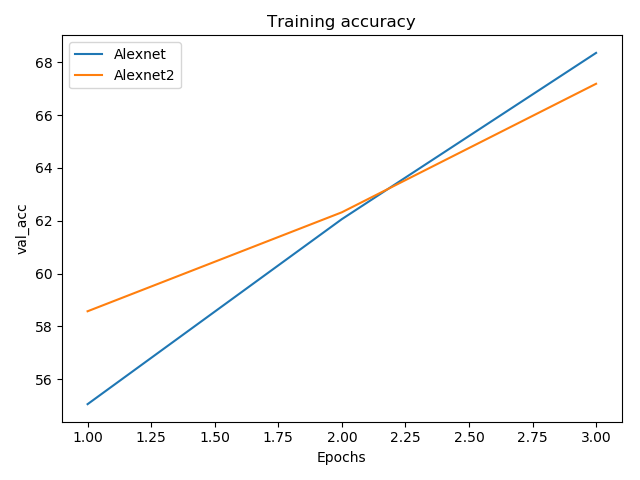
\includegraphics[width=25cm, height=15cm]{figures/prune_ratio}
\end{center}

This graph compare various level of pruning. Each level of pruning is made on two iteration made after 10 epochs of training and 3 epochs or retraining. Pretrained weight were used to see the impact on transfer learning.
}

\column{0.30}
\block{Comparing Pruning on  Multiple Models}{
	
	\vspace{-15pt}
	
\begin{center}
	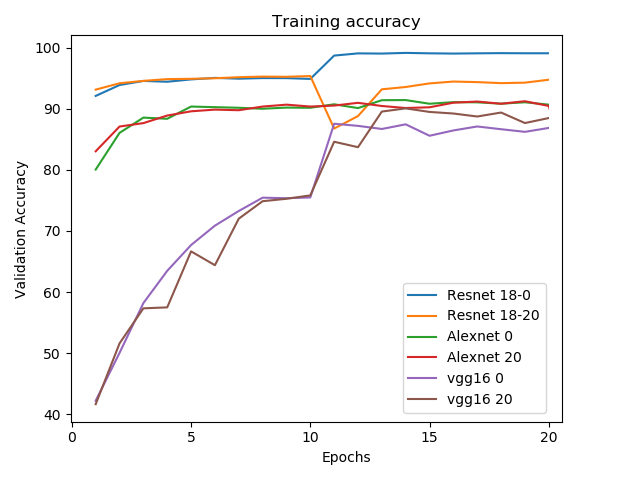
\includegraphics[width=25cm, height=15cm]{figures/various_models}
\end{center}

This graph explore the effect of pruning on different models. Each model shows the effect of pruning 20\% of the convolution filters in one step after 10 epochs of training.
}
\end{columns}

\begin{columns}
\column{0.50}
\block{Example of Network Reduction}{
	
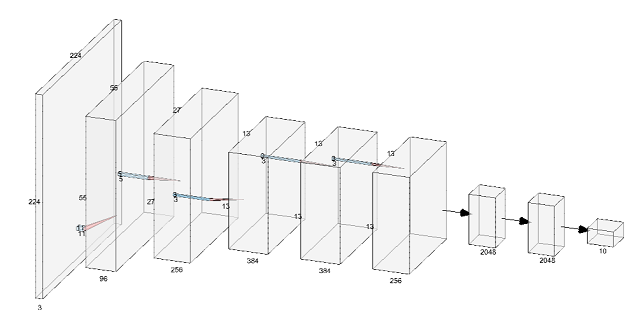
\includegraphics{figures/Alexnet_origin}
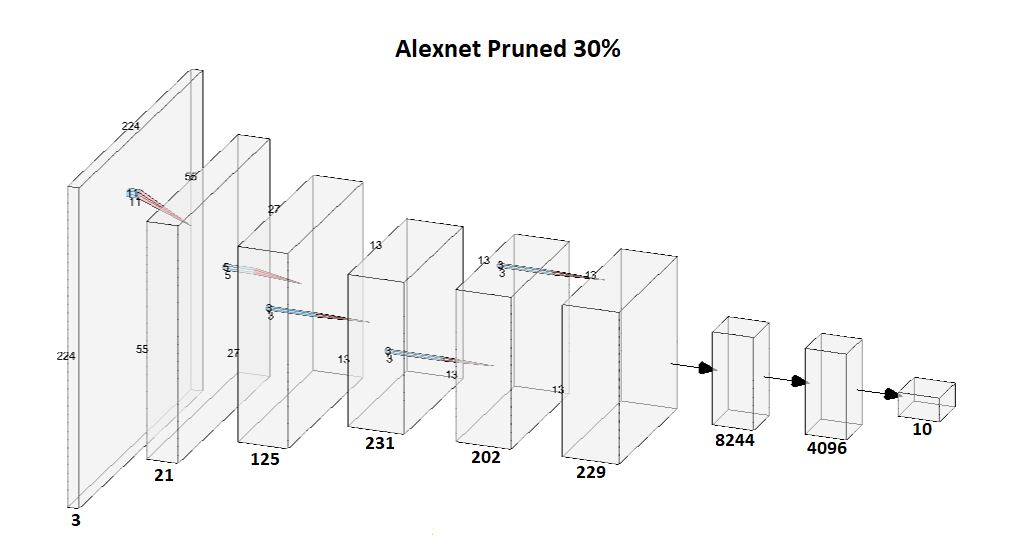
\includegraphics{figures/Alexnet_30}
	
	Comparing the effect of pruning on AlexNet. Left is the original model provided by pytorch. On the right is alex net pruned 30\%. In the case of network like Alexnet there is an important reduction of parameters based on the reduction of the fully connected layer. Their is also an important reduction in the first layers.
\vspace{41pt}
}


  \column{.25}
  \block{Algorithm}{
  	\begin{itemize}
  	\item Pretrain network with full paramters
  	\item \textbf{Prepare pruning}
  	\begin{itemize}
  	\item Convert model to ONNX
  	\item Extract execution graph
  	\item Determine which layer can be pruned
    \end{itemize}
  	\item \textbf{Prune network}
  	\begin{itemize}
  		\item Find number of filter to prune on iteration
  		\item Wort filter based on activation mean
  		\item Remove filters
  		\item Apply pruning effect to next layers
  		\item Reset optimizer
  	\end{itemize}
  	\item Finalize training
  \end{itemize}
  }

  \column{.25}
\block{Settings}{
	\textbf{Common:}
	\begin{itemize}
		\item \textbf{Optimizer}: Stochastic Gradient Descent
		\item \textbf{Learning Rate}: 0.01
		\item \textbf{Momentum}: 0.0
		\item \textbf{Nesterov}: False
		\item \textbf{Batch Size}: 64
		\item \textbf{Use GPU}: Yes
	\end{itemize}
\textbf{Pruning:}
\begin{itemize}
	\item \textbf{Pretrain Epoch}:  10
	\item \textbf{Retrain Epoch}: 3
	\item \textbf{Total nb. Epoch}: 20
\end{itemize}
\item \textbf{Nb Iteration on Alexnet}:  2
\item \textbf{Nb Iteration on Model Compare}:  1
\vspace{-4pt}
}

\end{columns}


\begin{columns}

  \column{.3}
  \block{Performances}{
  % \vspace{3mm}
\begin{center}
	\textbf{Comparing Alexnet Attributes after Pruning}
\begin{tabular}{c|c|cc|cc|cc|cc}
	& \textbf{0\%} & \multicolumn{2}{c|}{\textbf{10\%}}       & \multicolumn{2}{c|}{\textbf{30\%}}       & \multicolumn{2}{c|}{\textbf{50\%}}       & \multicolumn{2}{c}{\textbf{75\%}}        \\ \hline
	\textbf{FLOPs(G)}  & 0.815        & 0.665 & {\color[HTML]{009901} (-18.4\%)} & 0.445 & {\color[HTML]{009901} (-45.3\%)} & 0.283 & {\color[HTML]{009901} (-65.3\%)} & 0.133 & {\color[HTML]{009901} (-83.7\%)} \\ \hline
	\textbf{Params(M)} & 57.0         & 54.8  & {\color[HTML]{009901} (-3.86\%)} & 47.3  & {\color[HTML]{009901} (-17.0\%)} & 37.6  & {\color[HTML]{009901} (-34.0\%)} & 27.0  & {\color[HTML]{009901} (-52.6\%)}
\end{tabular}
\end{center}
  \vspace{-.5mm}
  }


  \column{.3}
  \block{Observations}
  {
  	\begin{itemize}
   \item Not all convolutional layer can be pruned. Pruning layer before a residual connection is dangerous because both side of the residual connection must have the same side.
  \item When pruning in a convolution layer it is important to propagate. So the next layer have the right input size. This apply to convolution, linear and batchnorm layers.
  \item The algorithm used tend prefer removing filters that are deeper in the model and it is not uncommon to try to prune all filter in a layer.
  \item When pruning it is important to reset optimizer.
  \end{itemize}
  }

  \column{.4} 
  \block{Conclusion}{
  
  \textbf{Discussion:}
    \begin{itemize}
        \item \colorbold{Morphology} and \colorbold{context} help predict useful embeddings.
        \item \colorbold{The attention mechanism works}: depending on the task, the network will use either more the context or the morphology to generate an embedding.
    \end{itemize}
    
    \textbf{Future works:}
    \begin{itemize}
        \item  Apply the \colorbold{attention mechanism on each character of the OOV word and each word of the context} instead of using the hidden state of the respective elements only.
        \item Test our attention model in \colorbold{different languages} and on other NLP tasks, such as \colorbold{machine translation}.
    \end{itemize}
    \vspace{-3.5mm}
  }
\end{columns}

\end{document}
